\subsection{a}
Given that $j^\alpha$ is a positive imaginary number, we can conclude that its argument is $\frac{\pi}{2}$, that is
\begin{equation}
\begin{split}
	&{(r e^{jx})}^\alpha = r^\alpha \left( \cos(x\alpha) + j\sin(x\alpha) \right) \quad \text{(De Moivre's theorem)}\\
	&j^\alpha =r^\alpha e^{jx\alpha} \implies x=\frac{\pi}{2}; r = 1\\
	&\therefore j^\alpha = e^{ j\frac{\pi\alpha}{2} } = \cos\left(\frac{\alpha\pi}{2}\right) + j\sin\left(\frac{\alpha\pi}{2}\right)
\end{split}
\end{equation}
\subsection{b}
\begin{equation}
\begin{split}
	Z &= R_\infty + \frac{R_0 - R_\infty}{1 + (j\omega\tau)^\alpha} \quad  \ \ = R_\infty + \frac{
		R_0 - R_\infty
		}{
			1 + (\omega\tau)^\alpha \cdot j^\alpha
		} \\
	&= R_\infty + \frac{
		R_0 - R_\infty
		}{
			1 + \theta^\alpha  \left(c + js\right)
			}
	= R_\infty + \frac{
			R_0 - R_\infty
		}{
			1 + \theta^\alpha c + \theta^\alpha js
		} \\
	&= R_\infty + \frac{
			R_0 - R_\infty
		}{
			1 + \theta^\alpha c + \theta^\alpha js
		}
		\cdot \frac{
			1+c\theta^\alpha - js\theta^\alpha
		}{
			1+c\theta^\alpha - js\theta^\alpha
		} \\
	&= R_\infty + \frac{
			\left( R_0 - R_\infty \right) \left( 1+c\theta^\alpha - js\theta^\alpha \right)
		}{
			1 + c\theta^\alpha + \cancel{js\theta^\alpha} + c\theta^\alpha + c^2\theta^{2\alpha} + \cancel{cjs\theta^{2\alpha}} - \cancel{js\theta^\alpha} - \cancel{jsc\theta^{2\alpha}} - {(js)}^2\theta^{2\alpha}
		} \\
	&= R_\infty + \frac{
		\left( R_0 - R_\infty \right) \left( 1+c\theta^\alpha - js\theta^\alpha \right)
		}{
			1+ 2c\theta^\alpha + \theta^{2\alpha}\left( c^2 - j^2s^2 \right)
		} \\
	&=
		R_\infty + \frac{
		\left( R_0 - R_\infty \right) \left( 1+c\theta^\alpha - js\theta^\alpha \right)
		}{
			1+ 2c\theta^\alpha + \theta^{2\alpha}\cancelto{1}{\left( c^2 + s^2 \right)}
		}
		\quad \quad \left(
			\text{from} \cos^2(x) + \sin^2(x) = 1
		\right) \\
	\therefore Z &= R_\infty + \frac{
		\left( R_0 - R_\infty \right) \left( 1+c\theta^\alpha - js\theta^\alpha \right)
		}{
			1+ 2c\theta^\alpha + \theta^{2\alpha}
		}
	\quad \quad \text{ as required} 
\end{split}
\end{equation}
\subsection{c}
Given that $\Delta = R_0 - R_\infty$, and $q = 1+2c\theta^\alpha + \theta^{2\alpha}$,
\begin{equation}
\begin{split}
	&Z = R_\infty + \Delta \frac{
		1 + c\theta^\alpha - js\theta^\alpha
	}{
		q
	} \\
	&Z = R_\infty + \frac{
		\Delta + \Delta c\theta^\alpha
	}{
		q
	}
	-j \frac{
		s\Delta\theta^\alpha
	}{
		q
	} \\
	&\implies |Z| =  \sqrt{
		{
			\left(
				R_\infty + \frac{\Delta + \Delta c\theta^\alpha}{q}
			\right)
		}^2
		+
		{
			\left(
				\frac{s\Delta\theta^\alpha}{q}
			\right)
		}^2
	} \\
	&|Z| = \sqrt{
	R_\infty^2 +
	\frac{
		2R_\infty\Delta + 2R_\infty \Delta c\theta^\alpha
	}{
		q
	} +
	\frac{\Delta^2 + 2\Delta^2c\theta^\alpha + \Delta^2c^2\theta^{2\alpha}}{q^2}
	+
		\frac{ {(s\Delta\theta^\alpha)}^2 }{q^2}
	} \\
	&  \left[\text{note that }
		\theta^{2\alpha}\Delta^2 \left(
			c^2 +s^2
		 \right)
	= \theta^{2\alpha}\Delta^2
	\right] \\
	&|Z|= \sqrt{
		R_\infty^2 +
		\frac{
			2R_\infty\Delta + 2R_\infty \Delta c\theta^\alpha
		}{
				q
		} +
		\Delta^2
		\cancelto{
			\frac{1}{q}
		}{
			\left(
				\frac{ 1 + 2c\theta^\alpha + \theta^{2\alpha} }{q^2}
			\right)
		}
	} \\
	& |Z|= \sqrt{
			\frac{
				qR_\infty^2+ 2R_\infty\Delta + 2R_\infty \Delta c\theta^\alpha
		+ \Delta^2
		}{
			q
		}
	} \\
	& |Z|= \sqrt{
		\frac{
			(1+2c\theta^\alpha + \theta^{2\alpha})R_\infty^2+ 2R_\infty (R_0 - R_\infty) + 2R_\infty (R_0 - R_\infty) c\theta^\alpha
	+ (R_0 - R_\infty)^2
	}{
		1+2c\theta^\alpha + \theta^{2\alpha}
	}
} \\
	&|Z|= \sqrt{
		\frac{
		\cancel{R_\infty^2} + \cancel{2c\theta^\alpha R_\infty^2} + R_\infty^2\theta^{2\alpha} + 
		\cancel{2R_\infty R_0} - \cancel{2R_\infty^2}+
		2R_\infty R_0c\theta^\alpha - \cancel{2R_\infty^2c\theta^\alpha}
		+ R_0^2 + \cancel{R_\infty^2} - \cancel{2R_0R_\infty}
		}
		{1+2c\theta^\alpha + \theta^{2\alpha}
		}
	} \\
	&\therefore  |Z| = \sqrt{
		\frac{
			R_\infty^2\theta^{2\alpha} +
			2cR_\infty R_0 \theta^\alpha +
			R_0^2
		}{
			1+2c\theta^\alpha + \theta^{2\alpha}
		}
	} \quad \text{ as required}
\end{split}
\end{equation}
\subsection{d}
\begin{figure}[h]
    \centering
    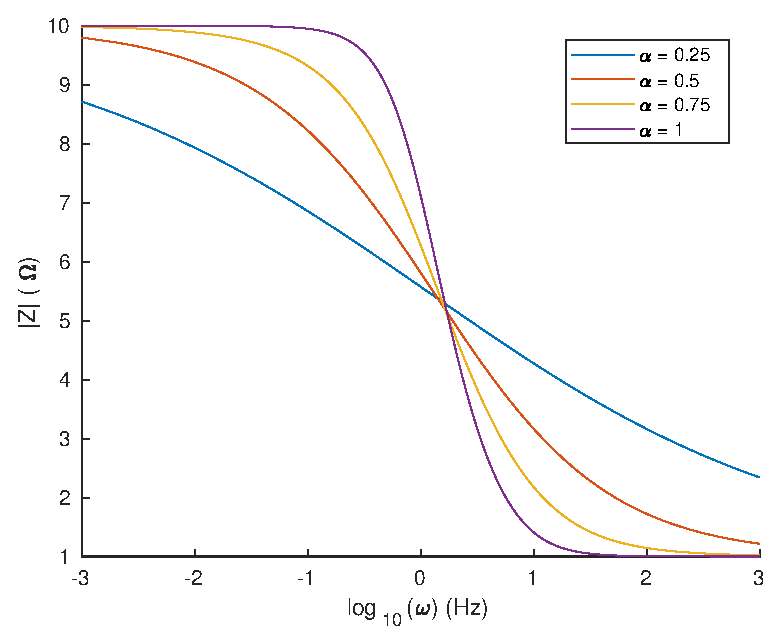
\includegraphics[scale=0.9, center]{./eps/topic4_d.eps}
    \caption{Magnitude of impedance plotted against angular frequency}
    \label{fig:Topic4-d}
\end{figure}
\pagebreak
\lstinputlisting[caption={Code for Topic 4. Question d.}]{"./files/topic 4/d.m"}

\subsection{e}
We see variations of logistic curves, which is surprising, given that the equation for $|Z|$ is quite different from the standard $f(x)$, such that

\begin{equation}
	f(x) = \frac{L}{1+e^{-k(x-x_0)}}
\end{equation}

Nevertheless, for $\alpha = 1$, we are left with $|Z| = \sqrt{\frac{{\log(\omega)}^2 + 10^2}{1+{\log(\omega)}^2}}$